\documentclass{beamer}

% This file is a solution template for:

% - Giving a talk on some subject.
% - The talk is between 15min and 45min long.
% - Style is ornate.



% Copyright 2004 by Till Tantau <tantau@users.sourceforge.net>.
%
% In principle, this file can be redistributed and/or modified under
% the terms of the GNU Public License, version 2.
%
% However, this file is supposed to be a template to be modified
% for your own needs. For this reason, if you use this file as a
% template and not specifically distribute it as part of a another
% package/program, I grant the extra permission to freely copy and
% modify this file as you see fit and even to delete this copyright
% notice. 


\mode<presentation>
{
  \usetheme[height=12mm]{Rochester}
  % or ...%

  \setbeamercovered{transparent}
%  % or whatever (possibly just delete it)
}


\usepackage[brazil]{babel}
% or whatever

% or whatever
%\usepackage{graphics}
\usepackage{times}
\usepackage[utf8]{inputenc}
\usepackage{url}

\newcommand{\nektar}{\ensuremath{\mathcal{N}\varepsilon \kappa \tau \alpha r}}
\newcommand{\ordem}[1]{ \ensuremath{\mathcal{O}[#1]}}
\newcommand{\pr}[1]{\ensuremath{ \mathbf{#1}}}    % \pr vem de preto
\newcommand{\etal}{\emph{et al.}}
\newcommand{\jac}[4]{ \ensuremath{ P_{#2}^{#3,#4}(#1) }}
\newcommand{\der}[2]{\ensuremath{ \frac{\partial #1}{\partial #2}}}
\newcommand{\convect}[2]{\ensuremath{ #1 \cdot \nabla #2}}
\newcommand{\R}{\ensuremath{ Re }}
\newcommand{\St}{\ensuremath{ St }}
\newcommand{\cpb}{\ensuremath{ C_{pb}}}
\newcommand{\transf}[3]{\ensuremath{ \int_{-\infty}^\infty #3\: e^{i #2 #1}\: d #2}}
\newcommand\clrms{\ensuremath{\sqrt{\overline{C_L^2}}}}
\newcommand{\epseudo}{\ensuremath{ \epsilon-\text{pseudospectro}}}
\newcommand{\lra}{\ensuremath{\longrightarrow}}

\newcommand{\wt}[1]{\ensuremath{\widetilde{#1}}}
\newcommand{\mcal}[1]{\ensuremath{\mathcal{#1}}}

\newcommand{\ol}[1]{\ensuremath{\overline{#1}}}
\newcommand{\us}{\ensuremath{u_*}}

\newcommand{\p}[1]{\ensuremath{ \mathbf{#1}}}    % \pr vem de preto
\newcommand{\qrq}{\ensuremath{\quad\lra\quad}}
\newcommand{\qqrq}{\ensuremath{\qquad\lra\qquad}}
\newcommand{\pd}{\ensuremath{\partial}}
\newcommand{\bigO}[1]{\ensuremath{\mathcal{O}\left(#1\right)}}


\title{Modelos, Escalas e Semelhança}


\author{Paulo Jabardo}

\titlegraphic{
\includegraphics[width=4cm]{figuras/logo-ipt.png}}%}
%   \includegraphics[width=2cm]{fig
%}
\date{24-11-2023}





\begin{document}
\maketitle
\begin{frame}{Camada limite atmosférica}
  Como modelamos a camada limite atmosférica no túnel de vento???

  Começamos com as equações da atmosfera:

  Equação da quantidade de movimento:
  \[
  \frac{\partial U_i}{\partial t} + U_j\frac{\partial U_i}{\partial x_j} + 2\varepsilon_{ijk} U_k\Omega_j = -\frac{1}{\rho_0}\frac{\partial \delta P}{\partial x_i} + \frac{g}{T_0}\delta T \delta_{3i} + \nu \frac{\partial^2 U_i}{\partial x_k \partial x_k}
  \]
  Equação da continuidade:
  \[
  \frac{\partial U_i}{\partial x_i} = 0
  \]
  Equação da energia:
  \[
  \frac{\partial\delta T}{\partial t} + U_k \frac{\partial\delta T}{\partial x_k} = \kappa \frac{\partial^2\delta T}{\partial x_k \partial x_k}
  \]
    
\end{frame}

\begin{frame}{Hipóteses}
  \begin{enumerate}
  \item Atmosfera é composta de um gás ideal com composição constante
  \item Os desvios de pressão, temperatura e densidade são pequenos quando comparados com a atmosfera neutra (adiabática)
  \item A densidade é independente da flutuação de pressão
  \item Variações de $\nu$ e $\kappa$ são desprezíveis
  \item A geração dew calor devido a dissipação viscosa é desprezível
  \item Não existem fontes de quaisquer tipo
  \end{enumerate}
\end{frame}
\begin{frame}{Adimensionalização}
  \[ L, \qquad U_R, \qquad, \rho_R, \delta T_R, \Omega_R\]
  \[
  \begin{aligned}
    x_i' = \frac{x_i}{L}, \qquad &U_i' = \frac{U_i}{U_R} \\
    t' = \frac{U_R}{L}t, \qquad &\rho' = \frac{\rho_0}{\rho_R} \\
    \delta P' = \frac{\delta P}{\rho_R U_R^2}, \qquad & \delta T' = \frac{\delta T}{\delta T_R} \\
    \Omega_k' = \frac{\Omega_k}{\Omega_R} \qquad & \\
  \end{aligned}
  \]
  
      
\end{frame}


\begin{frame}{Equações adimensionais}
  \[
  \frac{\partial U'_i}{\partial t'} + U'_j\frac{\partial U'_i}{\partial x'_j} + \frac{2}{Ro}\varepsilon_{ijk} U'_k\Omega'_j = -\frac{1}{\rho'}\frac{\partial \delta P'}{\partial x'_i} + \frac{1}{Fr}\delta T' \delta_{3i} + \frac{1}{Re} \frac{\partial^2 U'_i}{\partial x'_k \partial x'_k}
  \]
  \[
  \frac{\partial U'_i}{\partial x'_i} = 0
  \]
  Equação da energia:
  \[
  \frac{\partial\delta T'}{\partial t'} + U'_k \frac{\partial\delta T'}{\partial x'_k} = \frac{1}{Pe} \frac{\partial^2\delta T'}{\partial x'_k \partial x'_k}
  \]
\end{frame}

\begin{frame}{Parâmetros adimensionais}
  \[
  \begin{aligned}
    Ro \equiv \frac{U_R}{L\Omega_R} \qquad &\text{Número de Rossby}\\
    Fr \equiv \frac{U_R}{\sqrt{g L \frac{\delta T_R}{T_0}}} \qquad &\text{Froude densimétrico}\\
      Re \equiv \frac{U_R L}{\nu} \qquad &\text{Número de Reynolds}\\
      Pe \equiv \frac{U_R L}{\kappa} \qquad &\text{Número de Peclet}\\
  \end{aligned}
  \]
\end{frame}

\begin{frame}{E se tivermos transporte de espécie química}
  \[
  \frac{\partial \chi}{\partial t} + U_k\frac{\partial\chi}{\partial x_k} = \alpha \frac{\partial^2\chi}{\partial x_k \partial x_k}
  \]
  Em forma adimensional
  \[
  \frac{\partial \chi'}{\partial t'} + U'_k\frac{\partial\chi'}{\partial x'_k} = \frac{1}{ReSc} \frac{\partial^2\chi'}{\partial x'_k \partial x'_k}
  \]
  onde
  \[
  Sc \equiv \frac{\nu}{\alpha}
  \]
  
\end{frame}

\begin{frame}{Semelhança}
Gostaríamos
  \[
  Re_m\equiv Re_p, \quad Fr_m\equiv Fr_p, \quad Ro_m = Ro_p, \quad Pe_m\equiv Pe_p, \quad Sc_m\equiv Sc_p
  \]

  Será que conseguimos satisfazer estes parâmetros? Quase impossível, e todos só construindo um modelo em escala de 1:1 no mesmo local, etc!

  Vamos analisar cada adimensional:
\end{frame}

\begin{frame}{Número de Rossby}
  \centering
  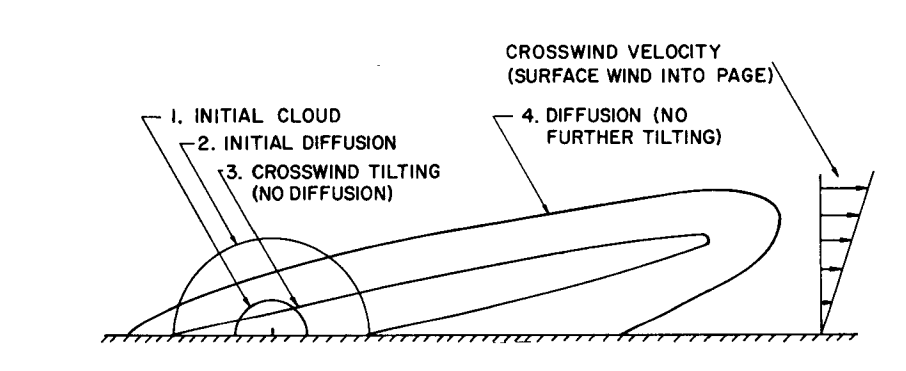
\includegraphics[width=\textwidth]{./figuras/coriolis.png}
\end{frame}



\begin{frame}{Rossby não é importante para escalas pequenas}
  Medições na atmosfera
\begin{itemize}
\item Domina o transporte para $L > 5\:km$
\item Desprezível para $L < 1\:km$
\end{itemize}

\emph{VAMOS DESPREZAR ISSO!!!}
\end{frame}


\begin{frame}{Número de Reynolds ($Re$)}
  \[
  Re_m \equiv Re_p \qrq \frac{U_m}{U_p} = \frac{L_p}{L_m} \times \frac{\nu_m}{\nu_p} \qrq \lambda_U =  \frac{1}{\lambda_L} \quad (\lambda_\nu\approx 1)
  \]
  Numa escala dimensional de 1:200, temos uma escala de velocidade de 200:1. Quase impossível!

  O quê fazer?
\end{frame}

\begin{frame}{Mecânica dos fluidos: a arte de ignorar Re e ser feliz}
  \centering
  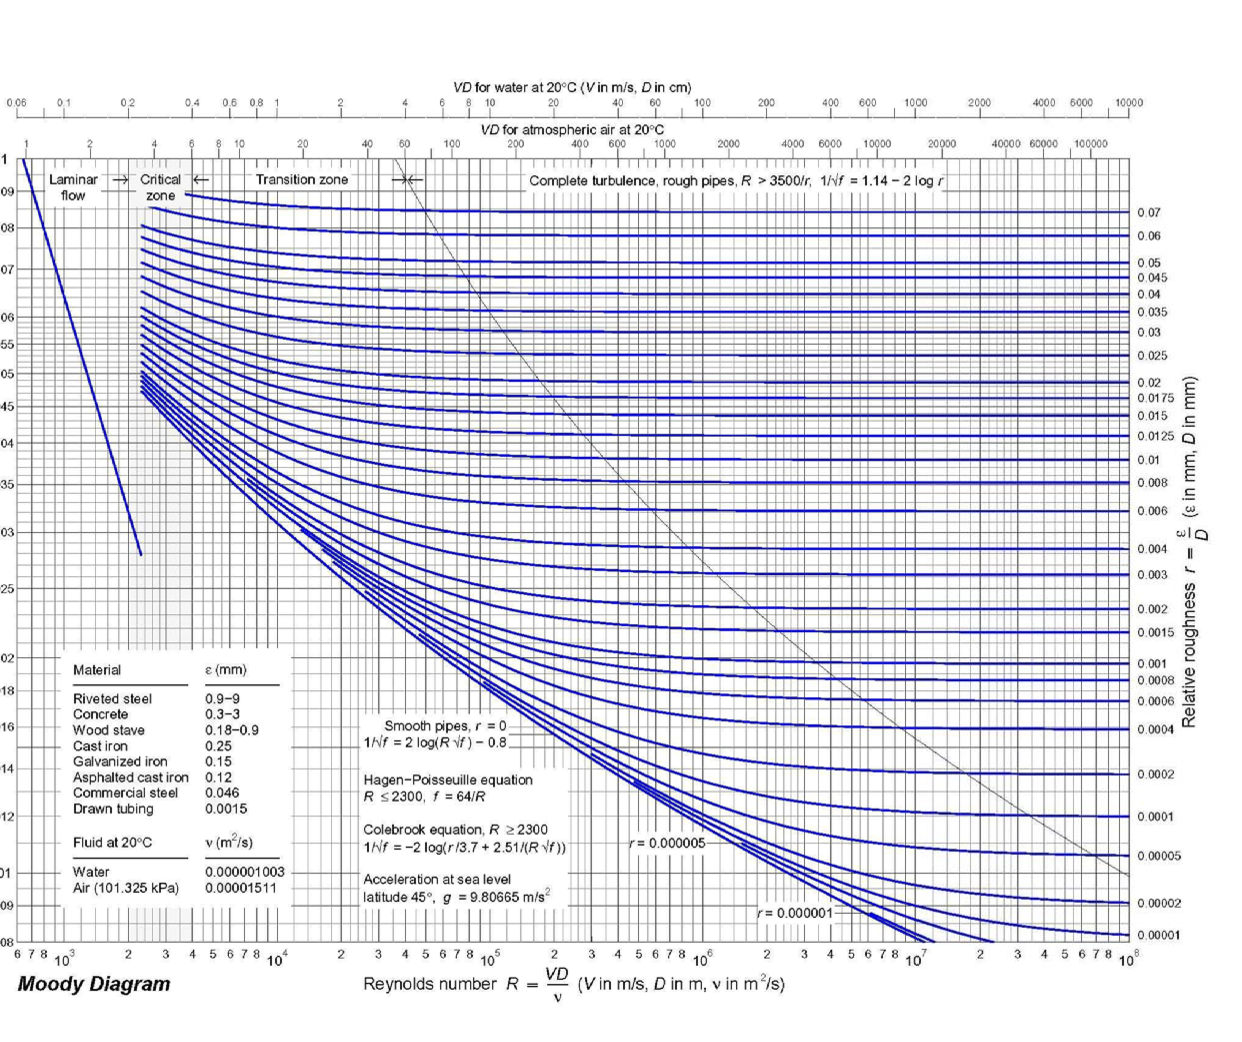
\includegraphics[width=0.9\textwidth]{./figuras/moody.pdf}
  
\end{frame}


\begin{frame}{Como Re afeta o escoamento?}
  \centering
  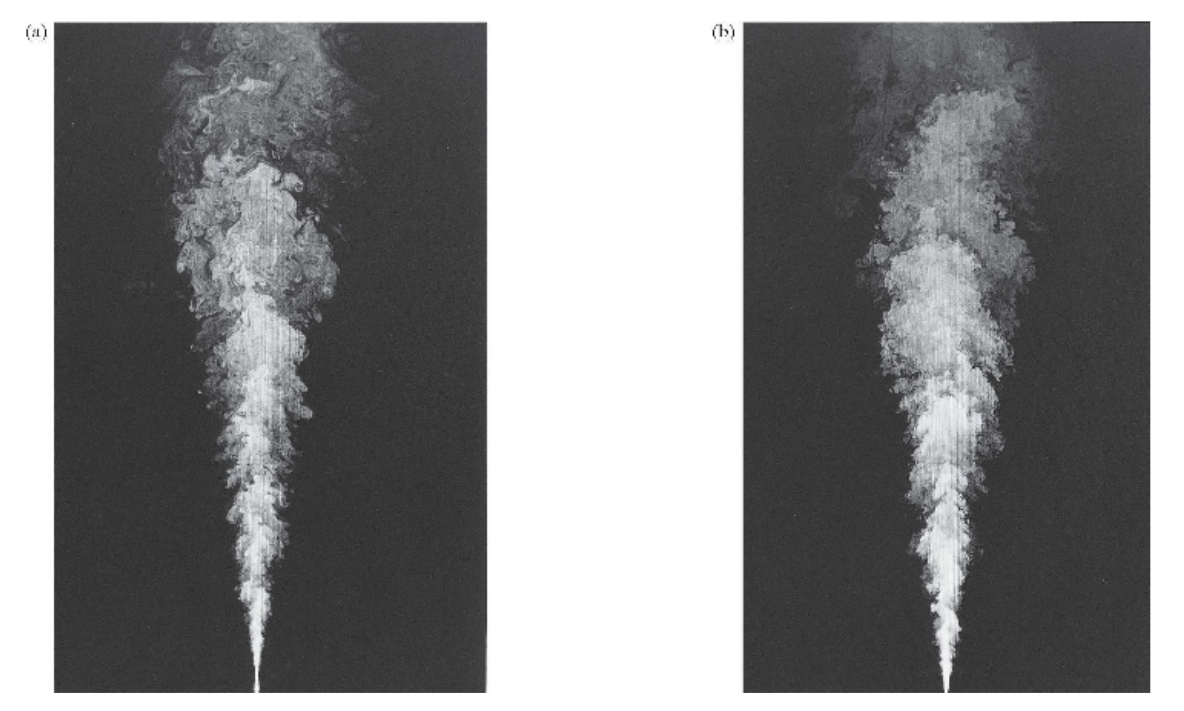
\includegraphics[width=\textwidth]{./figuras/jato-reynolds.png}
  
\end{frame}

\begin{frame}{Efeito de Re no espectro}
  \centering
  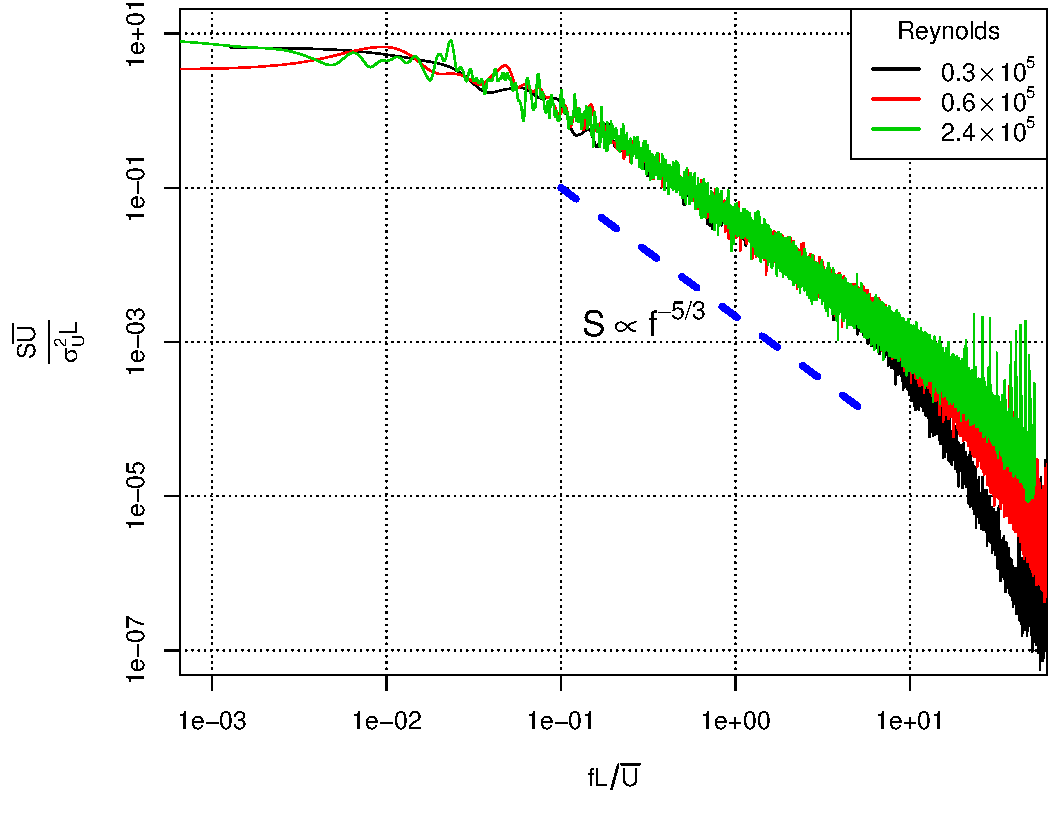
\includegraphics[width=0.9\textwidth]{./figuras/spec-nd.pdf}
  
\end{frame}

\begin{frame}{Como faremos?}
  \begin{itemize}
  \item Quanto maior Re menos importante ele é!
  \item Temos que garantir que Re seja alto o suficiente
  \item Lembre-se: escoamento não sabe fazer curva
  \item Curvas suaves: muito cuidado!!!
  \end{itemize}

\end{frame}


\begin{frame}{Qual Reynolds?}
  \centering
  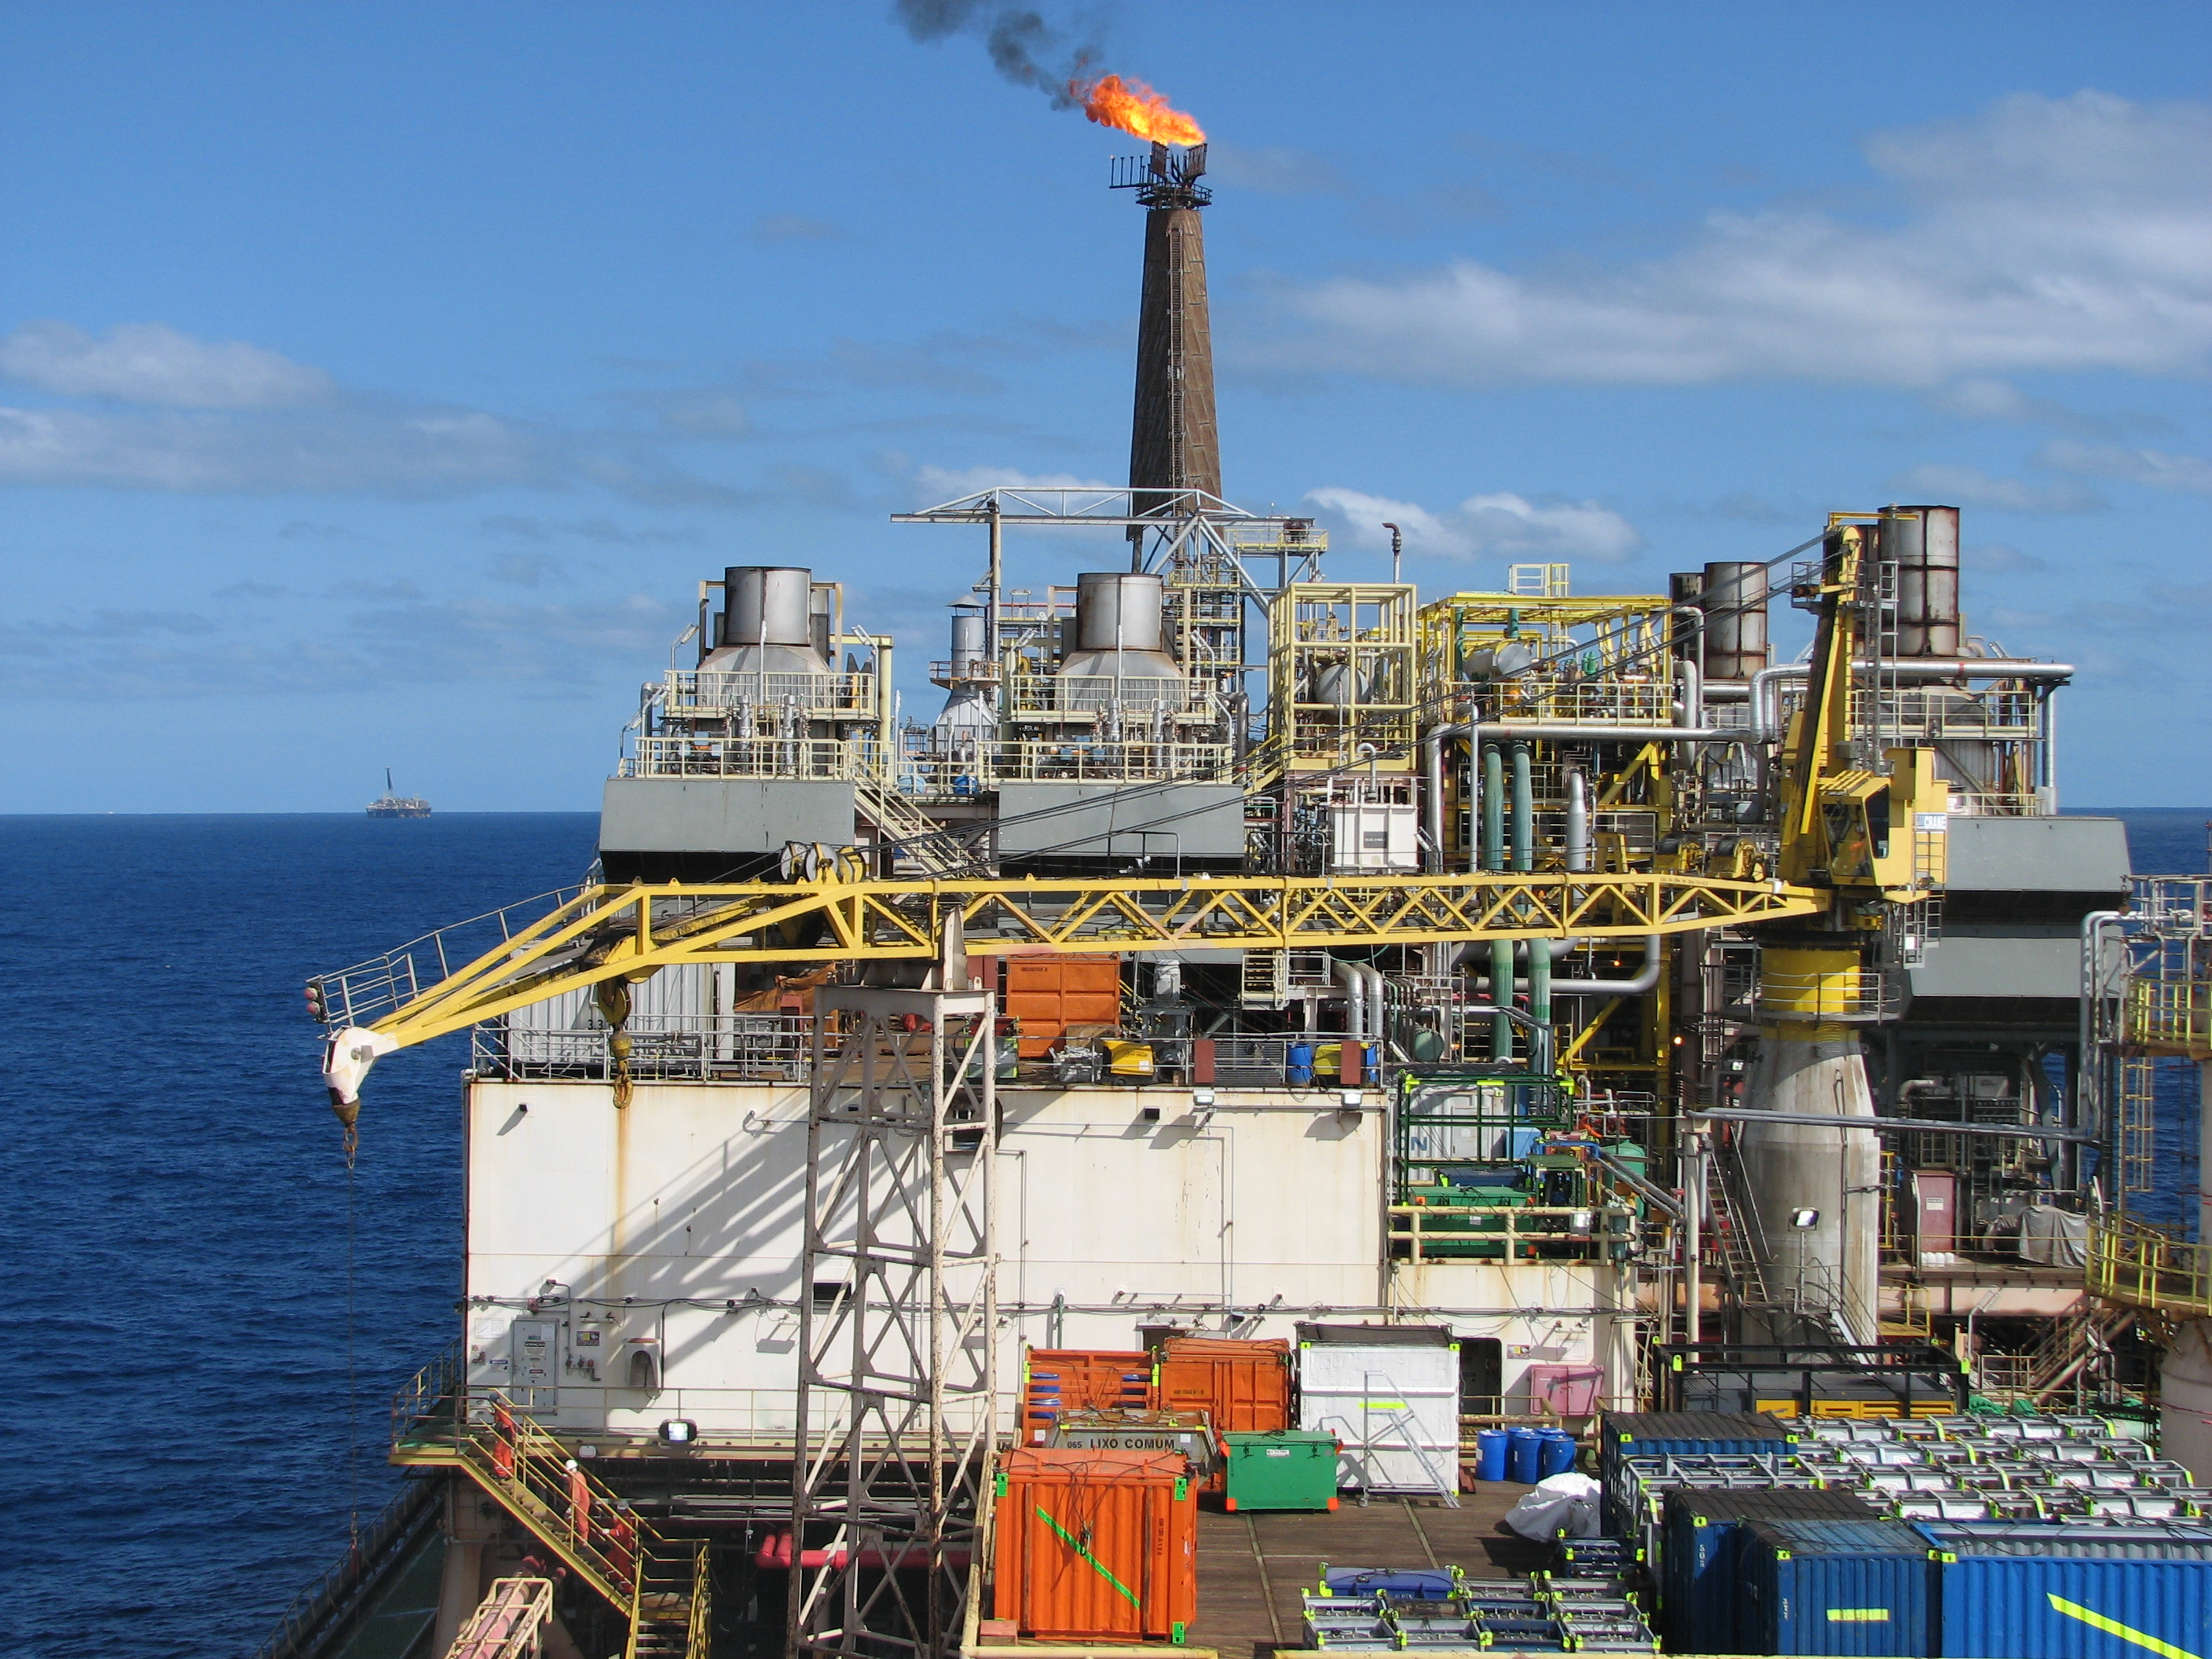
\includegraphics[width=\textwidth]{./figuras/foto-p37.jpg}
\end{frame}

\begin{frame}{Semelhança por coeficiente de arrasto}
  Elementos de pequenas dimensões com escoamento dependente de Re.
  \begin{itemize}
  \item Tubos e outros elementos estruturais
  \item Janelas, grades, etc
  \item Solução: distorcer escalas
  \end{itemize}

  Vamos usar uma escala dimensional diferente para o diâmetro
\end{frame}


\begin{frame}{Semelhança por coeficiente de arrasto}
  \centering
  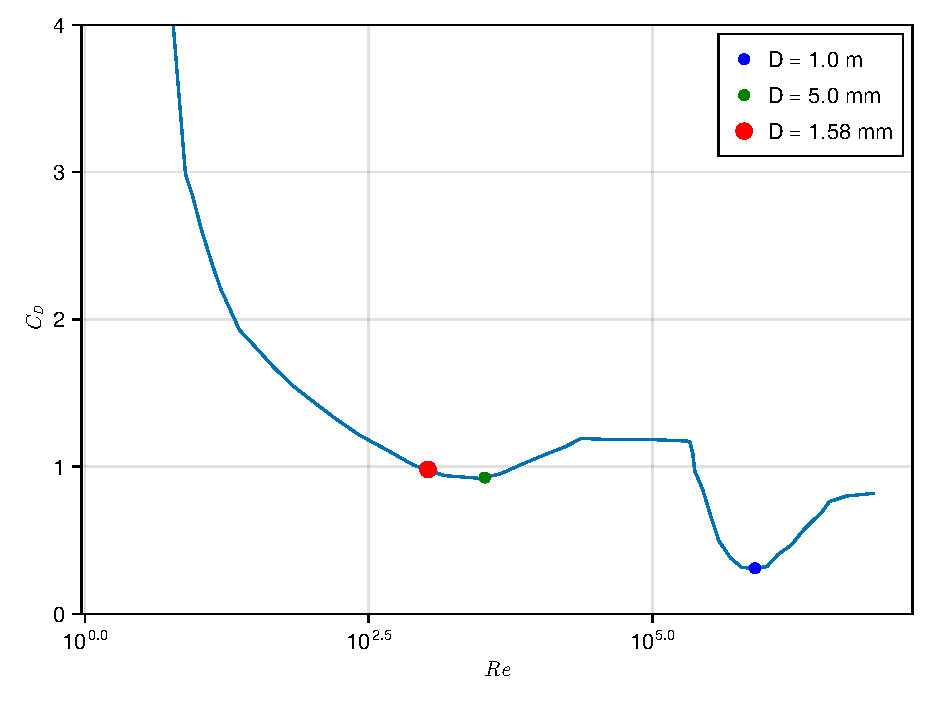
\includegraphics[width=\textwidth]{./figuras/cdsim.pdf}
\end{frame}



\begin{frame}{Froude densimétrico}
  Temos que reproduzir
  \[
  Fr = \frac{U_R}{\sqrt{g L \frac{\delta T_R}{T_0}}} \qquad \text{Froude densimétrico}
  \]

  Vamos admitir que
  \[
  \left.\frac{\delta T_R}{T_0}\right|_m =   \left.\frac{\delta T_R}{T_0}\right|_p
  \]

  Ou seja:
  \[
  \frac{U_{Rm}}{U_{Rp}} = \sqrt{ \frac{L_m}{L_p} } \qrq \lambda_U = \sqrt{\lambda_L}
  \]

  
  O que era ruim, piorou.
\end{frame}

\begin{frame}{Re muito baixo}
  \begin{itemize}
    \item Re já era baixo agora fica minúsculo
    \item Vai ter problema com Re
    \item Se $Re_p = 1\times 10^6$, $Re_m \approx 300$
    \item Escoamento dentro de chaminé é laminar
    \item Downwash
    \item Algumas possíveis soluções: contração, restrição
\end{itemize}
  
\end{frame}

\end{document}




\begin{frame}{}
\end{frame}


\begin{itemize}
\end{itemize}
